\documentclass[a4paper, 12pt]{article}
\usepackage{graphicx}
\usepackage{listings}

\setlength\parindent{24pt}

\lstset{language=c++,breaklines=true, frame=single}

\begin{document}

\begin{figure}
    \centering
    
\includegraphics[width=1\textwidth]{Logo}
\end{figure}

\title{Assignment Part 2 Report}
\author{Manwel Bugeja}
\date{\today}
\maketitle

\tableofcontents
\newpage

\section{Question 1}
\subsection{How the problem was tackled} 
For this part, "char" was added to the keyword\_type function within transitions.cpp. This was done so that "char" is identified as a keyword.
Apart from that, the square brackets where added to the transition tablle and classifier table. The states that the square brackets led to where added 
to the token\_type() function and to the list of accepting states. The updated part of the FSA is included as a figure.

\begin{figure}[h]
    \centering
    \frame{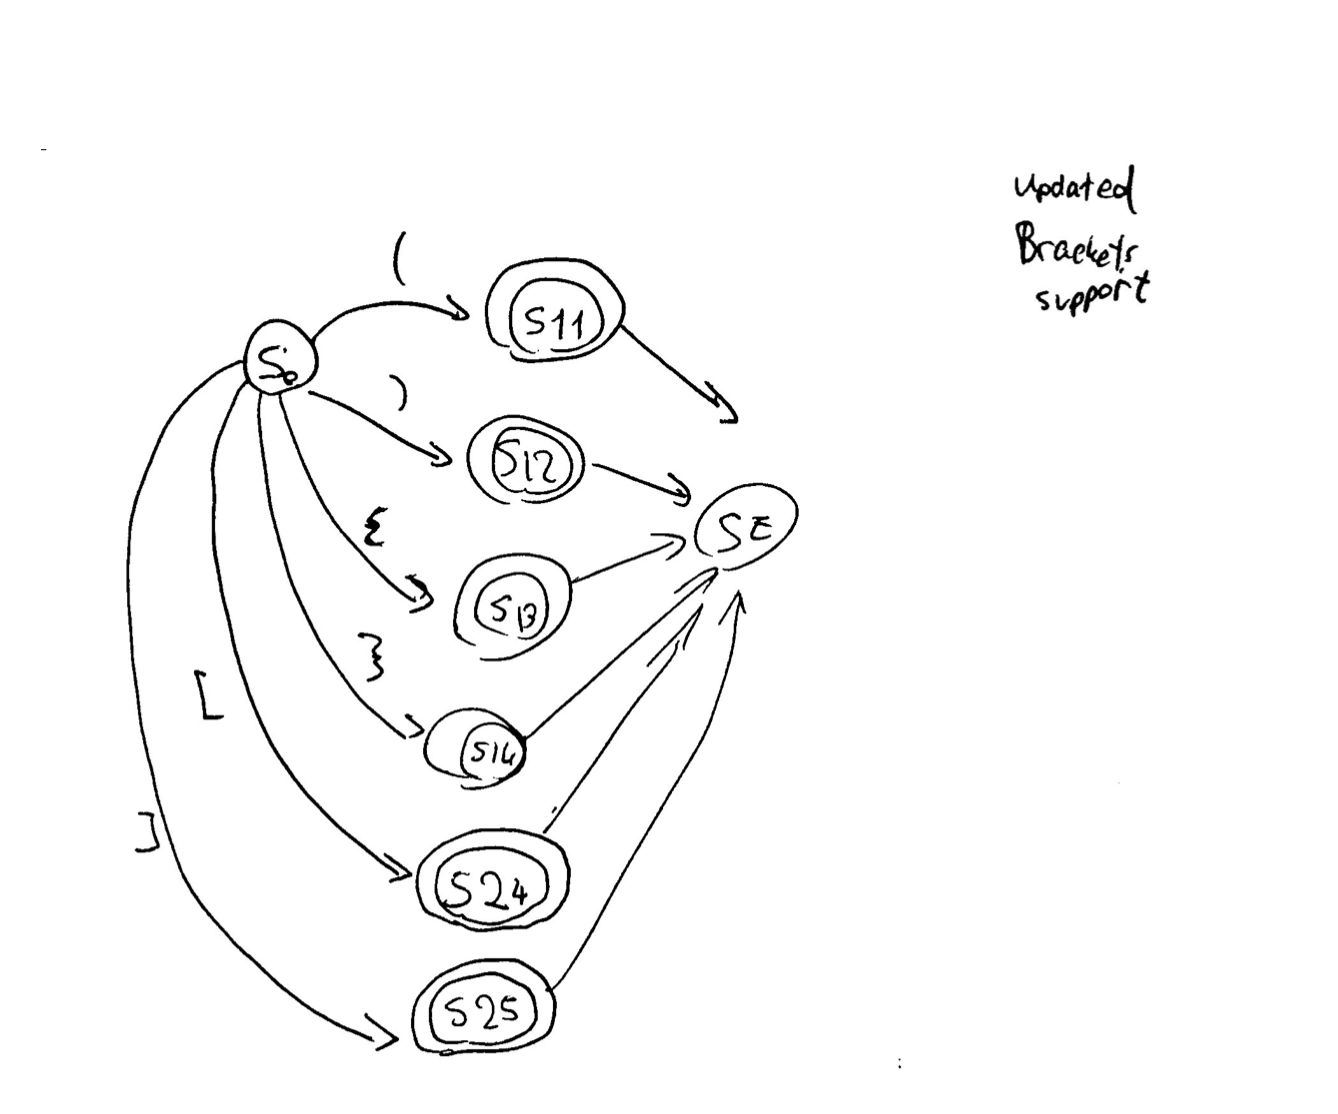
\includegraphics[width=1\textwidth]{images/brackets_updated}}
    \caption{FSA (part concerned with updated brackets)}
\end{figure}

\section{Question 2}
For this question, "char" was added to the function parse\_type(). This added support to initialize chars.
As for the array, a function was created according to the EBNF: "array ::= <identifier> '[' [ integerLiteral ] ']'"

The added function is listed as a figure. Furthermore, the array type was added tp the literal function.

\begin{lstlisting}[caption="Parsing arrays"]
AST* parse_array() {
    tell("array");
    AST* identifier_node = parse_identifier();
    if ( identifier_node == nullptr )   { return nullptr; }

    AST* l_square_node = parse_l_square();
    if ( l_square_node == nullptr )     { return nullptr; }

    AST* int_node = parse_integer_literal();

    AST* r_square_node = parse_r_square();
    if ( r_square_node == nullptr )     { return nullptr; }

    token new_token;
    new_token.type = array;
    return make_node(new_token, identifier_node, int_node);
}
\end{lstlisting}


\end{document}
